\section{Sprint 1}
\definecolor{gray}{gray}{0.6}

\subsection{Sprint Planning}
	The group planned a small delivery in this sprint, because we need time to set up the development environment and gain knowledge about the backbone framework and javascript, to make the implementations in the following sprints easier. During the sprint we will have the basis for the implementation ready such as models, views and presenters. The functional requirements concerning the map navigation and zooming are also to be implemented.

	In order to start implementing the other functional requirements, it requires that we have the map to put them on, and that all the elements in the game such as building, power plant and power line have been defined and implemented 

	To be able to keep up the testing activity in the upcoming sprints, we will try to get started with unit tests. This will probably take some time since testing is a new concept to many in the group as well as Jasmine is a new framework for all in the group. 

\subsection{Duration and workload}
	When the group had the firs meeting, we agreed to have sprints lasting for 2 weeks.
	After the 10 days into the first sprint, the group realized that goal was not reachable.
	The group decided to change the first sprint duration to 3 weeks instead of 2 weeks. \\

	{\bf Duration:} 09.09 - 29.09 (3 weeks)\\
	{\bf Workload:} This is the list with hours spent (the whole group) on the project in this sprint.
	\begin{itemize}
		\item {\bf Planning:} 11 hours
		\item {\bf Development:} 94,5 hours
		\item {\bf Design:} 14 hours
		\item {\bf Documentation (report):} 40,5 hours
		\item {\bf Testing:} 1 hour
	\end{itemize}
	{\bf Total workload: } 161 hours \\
	
	The group's goal was to work at least 20-25 hours pr/person every week. We did not manage this at this sprint, but we had a average of 13,5 hours/week (161 hours/4 persons/3 weeks = 13.5 hours). 
	In section 'problems during the sprint', we have written what have happened during this sprint.
	Many of the scenarios from that section affected the workload on the group. 

\subsection{Sprint backlog}
\begin{tabular}{| p{1cm} | p{8cm} | p{3cm} |}
	\hline
	\rowcolor{gray}
	ID & Description & Estimate \\ \hline
	FR2.1 & Buildings should appear around the map at arbitrary intervals and locations. & comment \\ \hline
	FR6.1 & The user should be able to see a small part of the game map. & comment \\ \hline
	FR6.2 & The user should be able to navigate around the map using the touch function on the phone & comment \\ \hline
	FR6.4 & The user should be able to view all of the map by double tapping the screen; double tapping a point on the complete map should zoom in on that area. & comment \\
	\hline
\end{tabular}

\subsection{Implementation}

\subsubsection*{Models}
	We have been using Backbone to implement the game models in this project. In Sprint 1 we have implemented 
	the following models to store game data.
	\begin{itemize}
		\item {\bf Building}
		The building model stores information about the buildings location on the game map as well as a reference 
		to the image that should be drawn on the map.
		\item {\bf Level}
		This model contains the map and player object. It is this object's job to handle the logic responsible for 
		updating the state of the game models.
		\item {\bf Map}
		The map model has two main functions. The first is to hold a Backbone Collection with all the buildings 
		that are placed on the map. The second is to maintain which part of the map that should be painted.
		\item {\bf Player} 
		The player model stores how many lives the player has and how much money the player has available to them.
	\end{itemize}

\subsubsection*{Presenters}
	Backbone Presenters are the JavaScript objects that connects the Backbone Models 
	to the visual HTML code. They listen to changes to the Backbone Models and changes 
	the HTML objects accordingly. The Presenters also handles input events from the HTML objects.
	
	\begin{itemize}
		\item {\bf Menu Screen}
		\item {\bf Game Screen}
		\item {\bf Instruction screen}
		\item {\bf Highscore screen}
	\end{itemize}
	\begin{figure}[H]
	\centering
	\subfigure{
		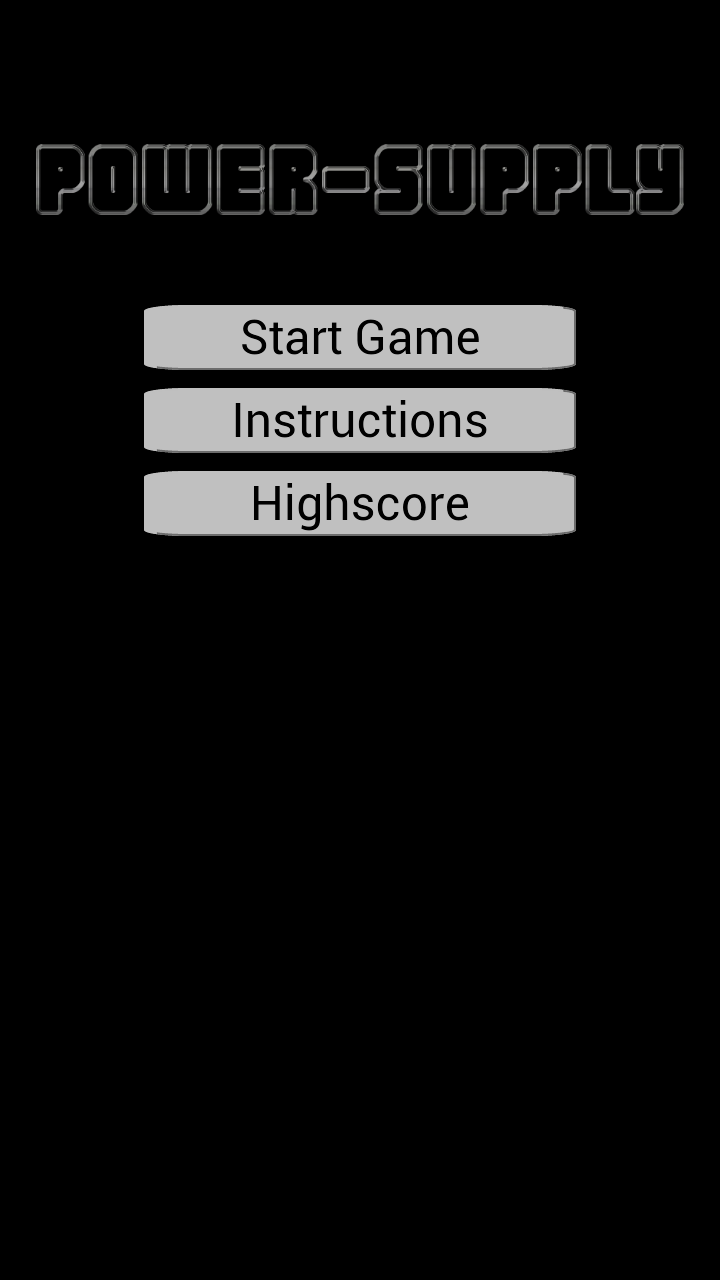
\includegraphics[scale=0.2]{pictures/game_screenshot_2}
	}
	\subfigure{
		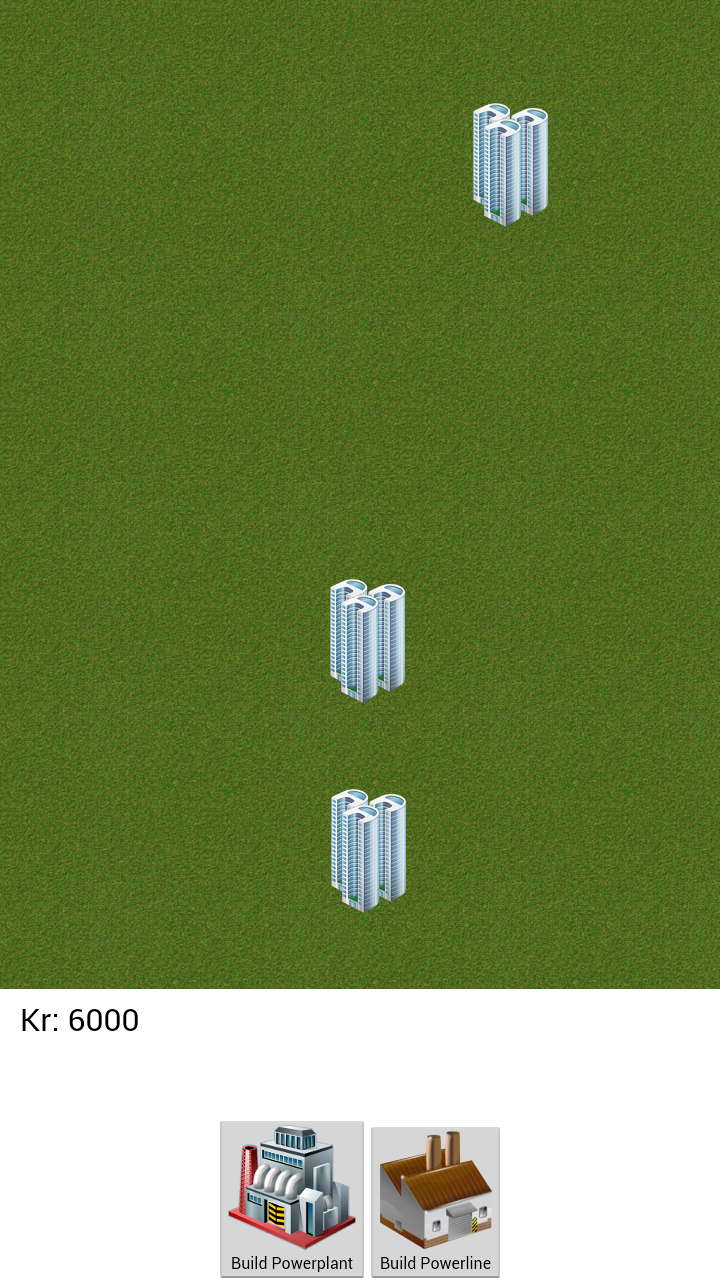
\includegraphics[scale=0.2]{pictures/game_screenshot_1}
	}
	\end{figure}

	\subsubsection*{Other Implementations}
		\begin{itemize}
			\item {\bf Place buildings on map}
			\item {\bf Rendering}
			\item {\bf Game Loop}
		\end{itemize}

\subsection{Testing}
	There has been minimal testing in the first sprint. Much time has been spent getting to know 
	the programming tools that are to be used and the focus has been on creating a base for further 
	programming as well as something more visual to show the customer, as opposed to planning tests 
	to be executed. The testing that has been carried out has been manual testing as well as 
	debugging using Android Debug Monitor. The manual testing has been carried out in parallel 
	with programming using an actual Android phone as well as Android Virtual Device. Android Virtual Device 
	is an emulator configuration that lets one model an actual device by defining hardware and 
	software options to be emulated. Functional tests for the implemented requirements took place at 
	the end of the sprint. The functional tests executed in this sprint were as follows:

\definecolor{lightgray}{gray}{0.9}

\begin{tabular}{| p{2cm} | p{7cm} | p{2cm} |}
	\hline
	\rowcolor{lightgray}
	{\bf Test Case} & {\bf Result} & {\bf Evaluation} \\ \hline
	FT-01 Map navigation & It is possible to move around the map as expected. When trying to move outside the map one stays in place in the outskirts of the map. & Pass. \\ \hline
  	FT-02 Appearance of buildings & Buildings do appear at regular intervals, within the map, but the rate at which they appear needs to be adjusted. It is also possible for a building to appear on top of another. & Still needs some corrections. \\ \hline
	FT-03 Zooming & Zooming is working as expected. When navigating fast the system sometimes interpret it as zooming. & Pass \\ \hline
\end{tabular}

\subsection{Group dynamics}
	In the start of this sprint we had a major problem that many of the group members was ill or 
	that many members didn't have the time to contribute to the project. 
	This is one of the risk factors 
	that we have listed in the risk analysis. 
	Apart form that, we had some problems with the group dynamics. The members in the group are 
	quite different and like to work in different ways. The main problem was 
	that many of the group members
	have different experiences with this kind of group work, technology as well as we have 
	different personalities.
	We managed to solve this problem by sitting down and discussing the problem. We discovered that
	one of the main problems was that the role allocation and the responsibility had not 
	been present.
	After we allocated the roles with a specific responsibility, many of our problems was solved and
	we have been able to work better as a group.

	Sprint 1 was the first phase in the project with implementation and coding. In the start, 
	many in the group had
	some problems with setting up the development environment (specially on windows). We managed
	to solve this problem, but it affected the total implementation because the whole group couldn't 
	contribute as much as we hoped. One solution was to go over from windows to ubuntu. 
	In the end of the sprint, everyone had a working development environment.

	Since no members in the group have a lot experience with the technology, it was sometimes hard
	to be able to do the implementations fast enough, or even know where to start. 
	Hopefully we will not have as much problems in the next sprints, but it is still a risk factor 
	since we are still quite inexperienced with javascript, mobile development and the framworks we use. 

\subsection{Customer feedback}
	In this sprint we did not get any feedback from the customer. We hope that the customer
	will get more involved in the next sprint. In the next sprint the group would like to have
	more feedback on the requirements. This is crucial because of the chosen working 
	methodology.

\subsection{Sprint retrospective}
	\subsubsection*{Start doing: } 
		\begin{itemize}
			\item require that the customer will give us feedback on the
			requirement specification in the next sprint.
			\item when one from the scrum team start implementing on a new feature, 
			it is a good practice to make a own branch in git for that. 
			\item always pull regularly from the master branch when developing
			on a own feature branch.
			\item start talking more to the other group members. This is crucial 
			for working together as a team.
		\end{itemize}
	\subsubsection*{Stop doing: } 
		\begin{itemize}
			\item stop coming late to the group appointments.
		\end{itemize}
	\subsubsection*{Continue doing: } 
